\newpage
\section{Aufbau}
Zentrale Elemente für den Versuch sind die zwei Laser welche auf eine Platte montiert sind. Die Platte selbst ist durchsichtig,
es bietet sich also an, einer Vielzahl an Messskalen variabel unter den Aufbau zu legen um so mehrere Messereihen mit der gleichen 
Konfiguration zu messen. \\
Die Laser selbst sind aufeinander monitiert, mit folglich horizontal versetzten aber parallelen Strahlen. Für verschiedene
Winkel bleibt es nun frei den Laser selbst oder das Medium mitsamt Messskala zu verschieben. Im uns dagegebenen Versuch 
ist eben der Laseraufbau variabel auf einem Kreisbogen mit einer Ausrichtung die immerzu auf das Medium zeigt. Der Laserstrahl 
bewegt sich also in Richtung des Normalenvektors des Kreisbogen bei entsprechender Position. 
\begin{figure}
    \centering
    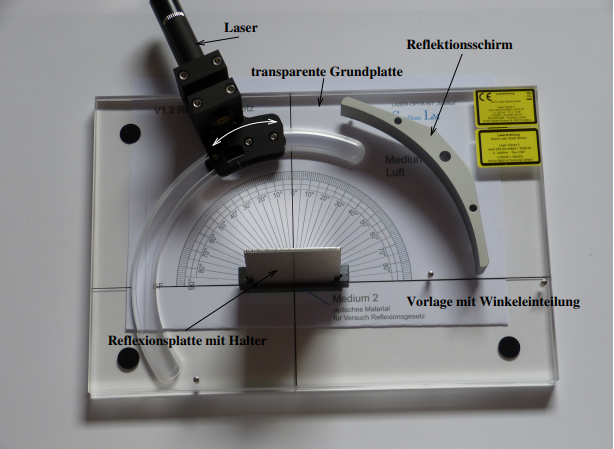
\includegraphics[width=0.5\textwidth]{bilder/afbau.png}
    \caption{Bildaufnahme der transparenten Platte mit montiertem Aufbau bestehend aus den Lasern, Medium und Reflektionsschirm.
    Deutlich erkennbar ist hier der Kreisbogen um das Zentrum auf dem der Laser frei verschiebbar ist. \cite{skript}} 
    \label{fig:teile}
\end{figure}
\FloatBarrier
\flushleft Im laufe der Durchführung wird sowohl Reflexion als auch Beugung beobachtet, es gilt also Werte jeweils hinter oder vor dem Medium 
aufzunehmen. Im Falle von Reflexion ist ein sogenannter Reflektionsschirm auf die Platte fixiert. Dieser bietet Halt für eventuelle
Transmissionsschirme oder allgemeinen Schutz vor dem Laserlicht.

Da Laser im allgemeinen eine enorm hohe Kohärenzlänge aufweisen, spielt der Abstand zum Medium keine weitere Rolle. 
Die Laserdiodenmodule erzeugen eine Wellenlänge von $\SI{635}{\nano\meter}$ für das rote und $\SI{532}{\nano\meter}$ für das
grüne Licht \cite{skript}.

\begin{figure}
    \centering
    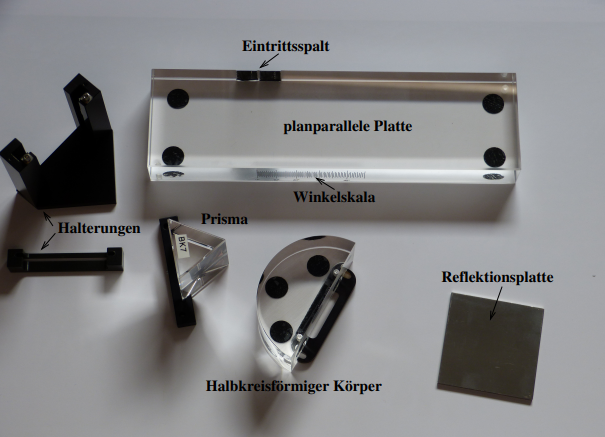
\includegraphics[width=0.5\textwidth]{bilder/teile.png}
    \caption{Bildaufnahme der verschieden Elemente die im Verlaufe des Versuchs V400 verwendet wurden. \cite{skript}} 
    \label{fig:teile}
\end{figure}
\FloatBarrier

Das optische Material, welches im Mittelpunkt des Kreisbogens zu platzieren ist, bedient sich verschiedener Elemente um 
die jeweils gesuchten Messwerte zu bestimmen. Bei manchen dieser Medien empfiehlt es sich eine enstprechende Haltung zu benutzen.
\begin{description}
    \label{idkwhatthisissss}
    \item Planparallele Platte: \\
    Dieses Element misst eine Dicke von $d = \SI{5.85}{\cm}$, weist auf einer Seite einen Eintrittsspalt und auf der anderen 
    eine Winkelskala auf.
    \item Prisma: \\
    Das Prisma besteht aus Kronglas und ist charakterisiert durch einen brechenden Winkel $\gamma = 60 \si{\degree}$.
    \item Reflektionsplatte: \label{lol}\\ 
    Um das Reflexionsgesetz zu verifizieren muss das Laserlicht nahezu perfekt refelektiert und anschließend der Winkel
    gemessen werden. Dazu wird die sogenannte Reflektionsplatte benutzt die das Licht mit einem Reflektionskoeffizienten $R ≃ 1$
    reflektiert.
\end{description}
\newpage
\section{Durchführung}
Vier verschiedene Konfigurationen werden für die Durchführung benötigt um die Gesetzte der Optik zu verifizieren.

\subsection{Reflexionsgesetz}
Zu Beginn wird mit Hilfe der Reflektionsplatte der Winkel von den ein - und ausfallenden Laserstrahlen des grünen Laser gemessen. 
Eine passende Messskala unter der Platte lässt den Winkel bei sieben verschiedenen Einfallswinkeln ablesen.

\subsection{Brechungsgesetz}
Die Reflektionsplatte wird mit der Platte getauscht. Aus der Natur der Brechung folgt, dass es jetzt Werte 
vor dem Medium zu Messen gilt, da hier das Laserlicht größtenteils Transmission erfährt.
Der verschiebbare Laseraufbau wird auch hier sieben mal auf seinem Kreisbogen verstellt, sodass der grüne Laser 
nach der Brechung auf der Winkelskala der Platte abzulesen ist. 

\subsection{Prisma}

Sowohl der rote als auch der grüne Laser leuchten hier auf das im Zentrum plazierte Prisma.
Eine Kreisförmige Winkelskala wird in dem Bereich aufgebaut, in dem anschließend das gebrochene Licht strahlt. Diese gibt Aufschluss
über die zu messene Ablenkung $\delta$ die das Licht durch das Prisma, bei fünf verschiedenen Einfallswinkeln $\alpha$ im Bereich von 
$\SI{10}{\degree} \leq \alpha_1 \leq \SI{60}{\degree}$ erfährt.
    \begin{figure}
        \centering
        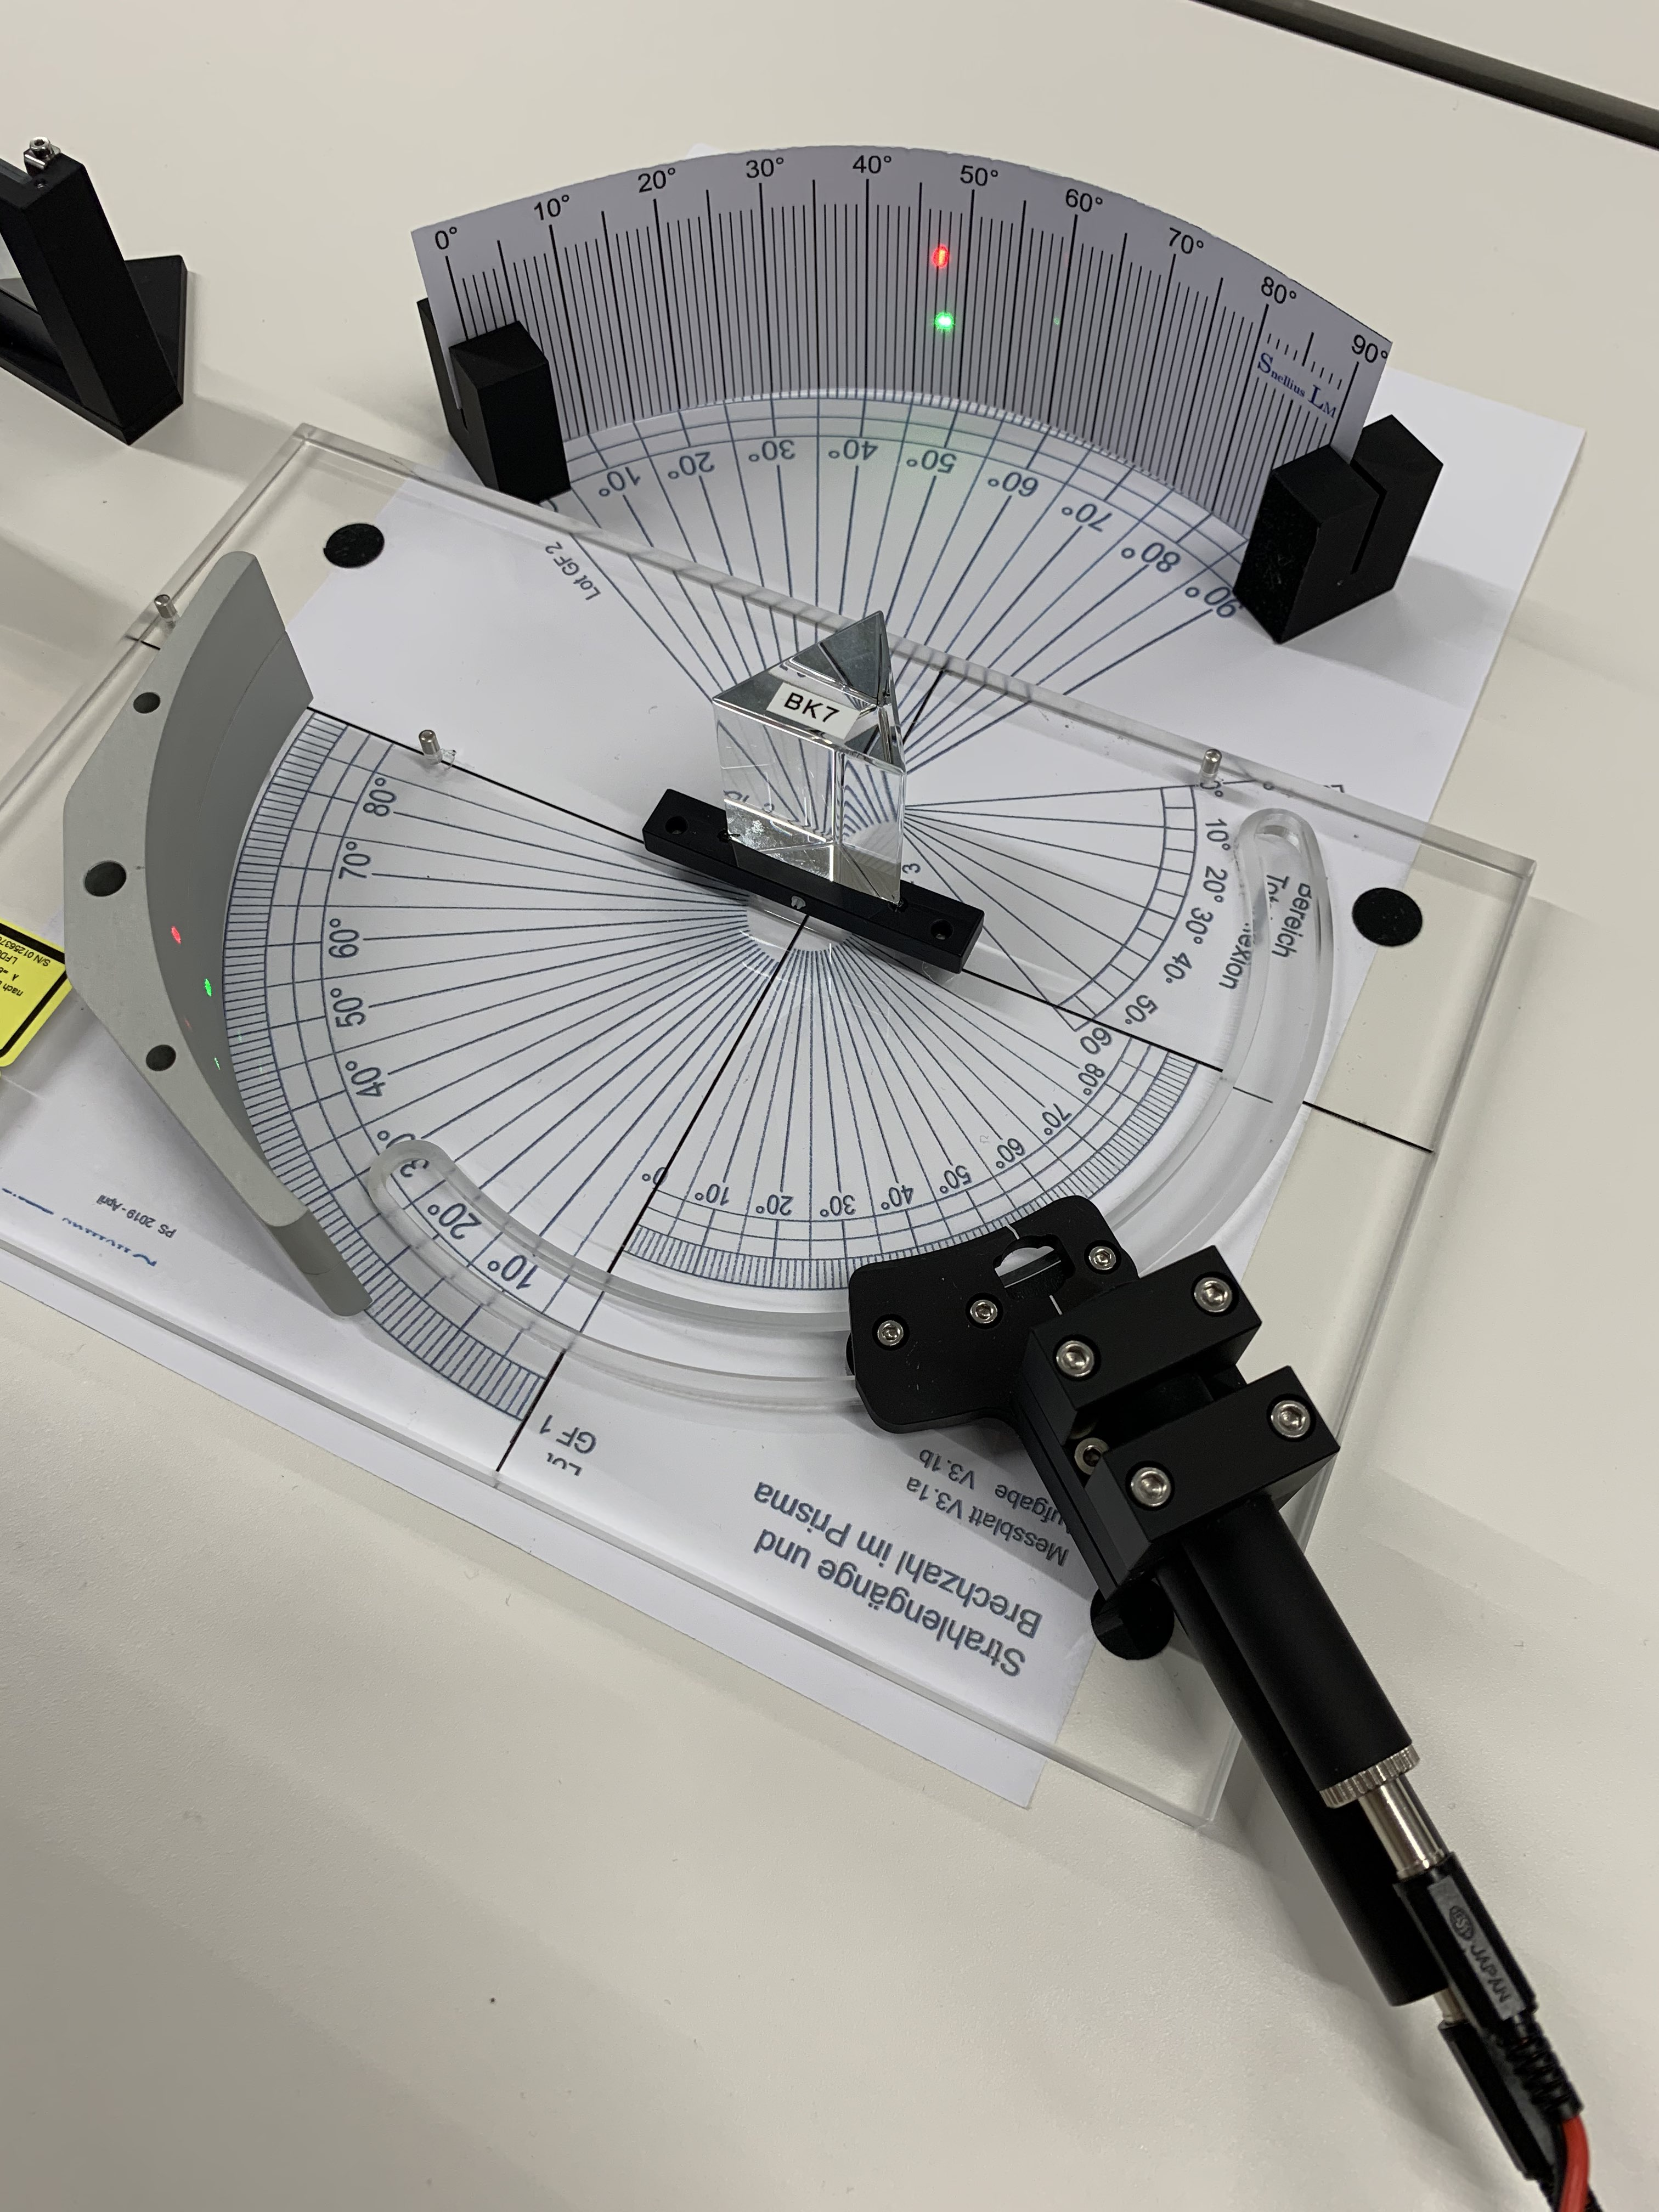
\includegraphics[width=0.3\textwidth]{bilder/prisma.jpg}
        \caption{Zu sehen ist eine Momentaufnahme des Aufbaus bei der Aufgabe 4. \cite{skript} 
        Klar erkennbar ist der totale Brechungswinkel auf der Winkelskala.}
\end{figure}
\newpage
\subsection{Beugung am Gitter}
Beide Laser strahlen bei dieser Messreihe auf ein in der Mitte platziertes Gitter. Dieses wird durch die Gitterdichte, also wie viele
Linien pro $\si{\milli\meter}$ auftreten, beschrieben. Zur verfügung stehen drei verschiede Dichten. 
\begin{align*}
    \SI{100}{Lines \per \milli\meter} \\
    \SI{300}{Lines \per \milli\meter} \\
    \SI{600}{Lines \per \milli\meter} 
\end{align*}
Die gesuchten Winkel der Interferenzmaxima lassen sich durch eine Winkelskala ablesen.
    \begin{figure}
        \centering
        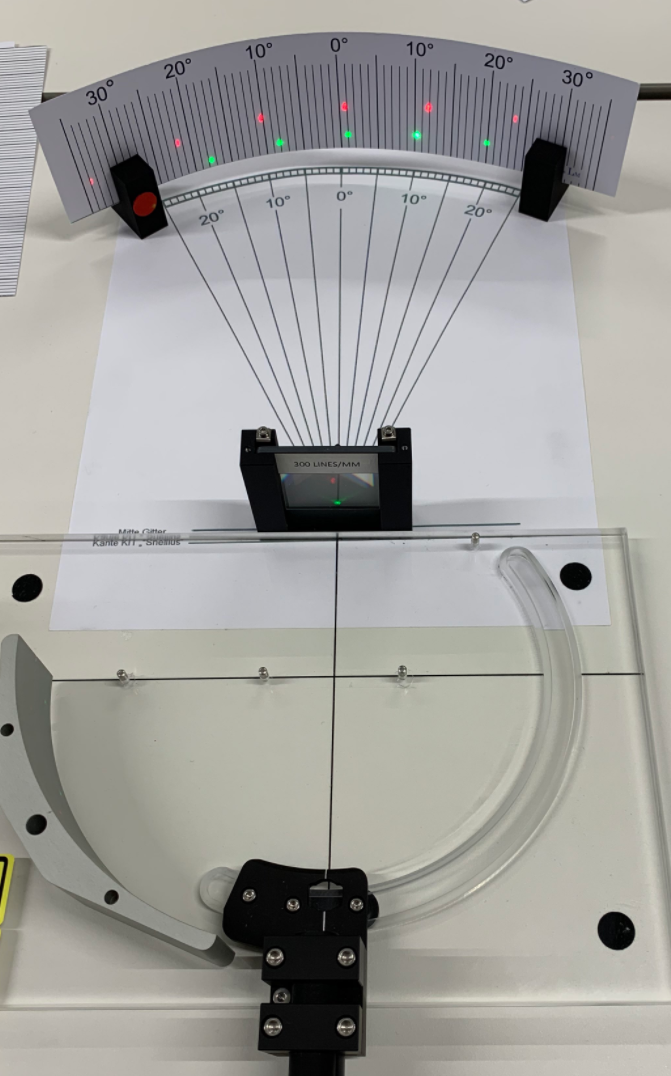
\includegraphics[width=0.3\textwidth]{bilder/gitter.png}
        \caption{Hier ist der Aufbau dargestellt um den Winkel zwischen den Interferenzmaxima bei einem Gitter
        (siehe Aufgabe 5 \cite{skript}) zu messen. Die Halterung verhindert, dass das Gitter direkt ins Zentrum gestellt werden kann.
        Die Kohärenzlänge des Lasers gewährleistet aber eine gewisse Invarianz bezüglich der Entfernung, wodurch keine Ergebnisse verfälscht werden.}
\end{figure}




